% F4 — The steering loop (Böckeler): incident -> prior art -> distiller -> lesson at the
% strongest feasible layer (code > hook > artifact > agent) -> register row with its origin ->
% a test that fails on recurrence -> the next burst runs a better pipeline; K clean passes -> freeze.
% Solid = DEPLOYED; dashed = PROPOSED. COLOUR GRAMMAR (PI 2026-09-03): blue = code, green = model role, white = documents,
% amber = the human decision; the enforcement-hierarchy ladder keeps its greys (it is a scale, not a set of actors).
\documentclass[tikz,border=4pt]{standalone}
\usepackage[T1]{fontenc}
\usepackage{lmodern}
\usetikzlibrary{positioning,calc,shapes.geometric,arrows.meta}
\newcommand{\nohyph}{\hyphenpenalty=10000 \exhyphenpenalty=10000 }
\definecolor{codefill}{RGB}{199,217,239}\definecolor{codeline}{RGB}{59,110,165}
\definecolor{agentfill}{RGB}{226,240,217}\definecolor{agentline}{RGB}{58,125,52}
\definecolor{humanfill}{RGB}{253,236,200}\definecolor{humanline}{RGB}{191,124,0}
\definecolor{docline}{RGB}{110,110,110}
\begin{document}
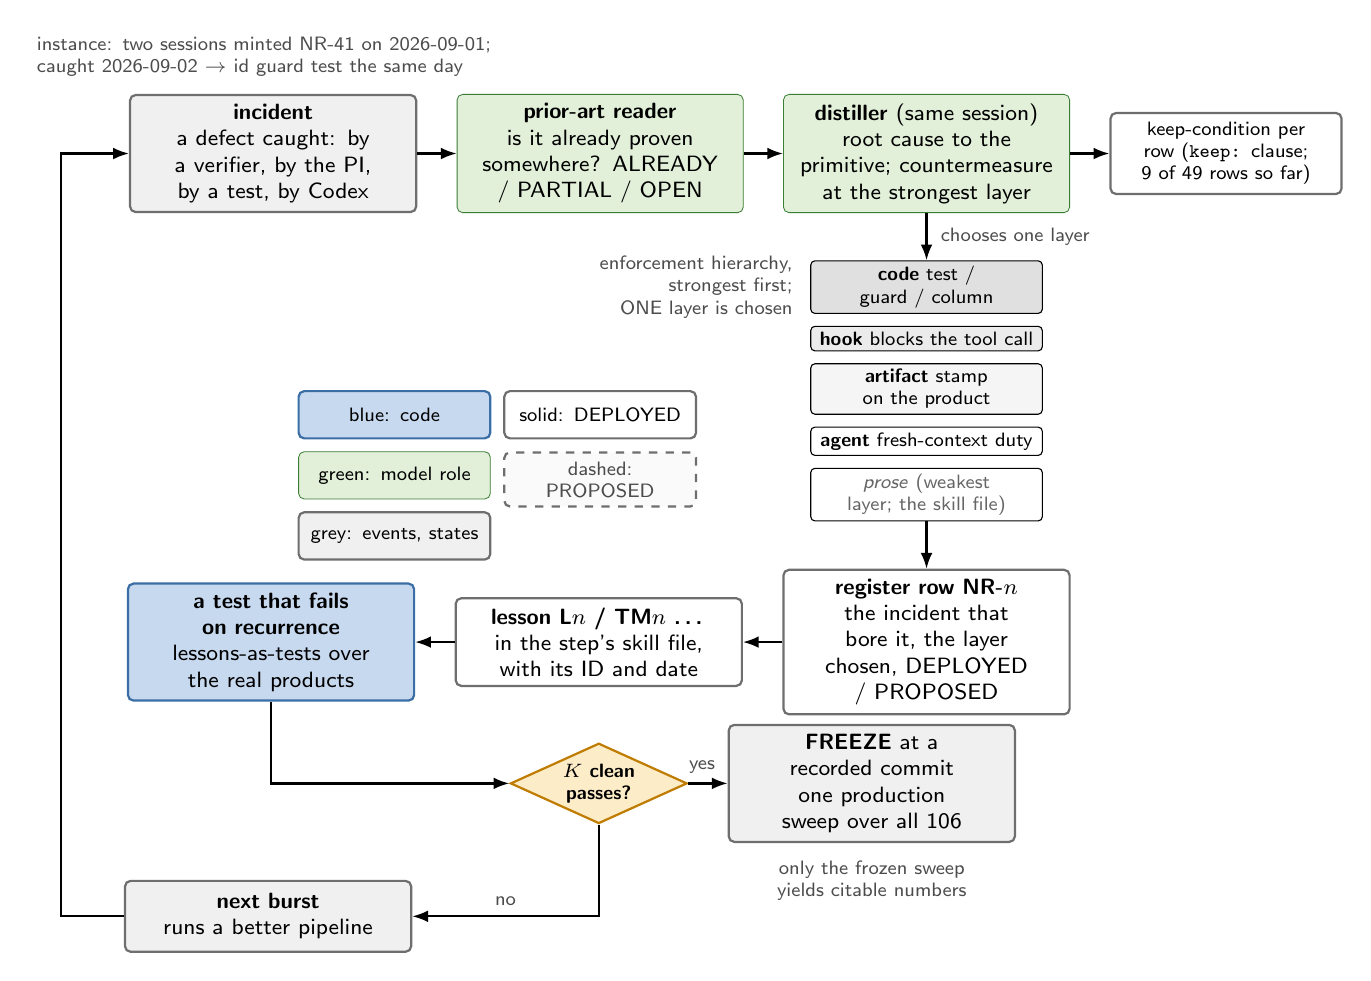
\begin{tikzpicture}[
  font=\sffamily\footnotesize, node distance=4mm and 5mm,
  box/.style={draw=docline, thick, rounded corners=2pt, fill=white, text width=34mm, align=center, minimum height=9mm, execute at begin node=\nohyph},
  code/.style={box, fill=codefill, draw=codeline, line width=0.8pt},
  agent/.style={box, fill=agentfill, draw=agentline, line width=0.3pt},
  event/.style={box, fill=black!6},
  prop/.style={box, dashed, fill=black!2, text=black!70},
  dec/.style={draw=humanline, thick, diamond, aspect=2.2, fill=humanfill, inner sep=1pt, align=center, font=\sffamily\scriptsize\bfseries},
  layer/.style={draw, rounded corners=1.5pt, text width=28mm, align=center, font=\sffamily\scriptsize, inner sep=2pt, execute at begin node=\nohyph},
  arr/.style={-{Latex[length=2mm]}, thick},
  lab/.style={font=\sffamily\scriptsize, text=black!70}]

\node[event] (inc) {\textbf{incident}\\a defect caught: by a verifier, by the PI, by a test, by Codex};
\node[agent, right=of inc] (prior) {\textbf{prior-art reader}\\is it already proven somewhere? ALREADY / PARTIAL / OPEN};
\node[agent, right=of prior] (dist) {\textbf{distiller} (same session)\\root cause to the primitive; countermeasure at the strongest layer};

% the enforcement hierarchy under the distiller
\node[layer, below=6mm of dist, fill=black!12] (L1) {\textbf{code} test / guard / column};
\node[layer, below=1.5mm of L1, fill=black!8] (L2) {\textbf{hook} blocks the tool call};
\node[layer, below=1.5mm of L2, fill=black!4] (L3) {\textbf{artifact} stamp on the product};
\node[layer, below=1.5mm of L3] (L4) {\textbf{agent} fresh-context duty};
\node[layer, below=1.5mm of L4, text=black!60] (L5) {\textit{prose} (weakest layer; the skill file)};
\node[lab, left=1mm of L1.west, anchor=east, text width=30mm, align=right, execute at begin node=\nohyph] {enforcement hierarchy, strongest first; ONE layer is chosen};

\node[box, below=6mm of L5] (reg) {\textbf{register row NR-$n$}\\the incident that bore it, the layer chosen, DEPLOYED / PROPOSED};
\node[box, left=of reg] (lesson) {\textbf{lesson L$n$ / TM$n$ \ldots}\\in the step's skill file, with its ID and date};
\node[code, left=of lesson] (test) {\textbf{a test that fails on recurrence}\\lessons-as-tests over the real products};

\node[dec, below=7mm of lesson] (k) {$K$ clean\\passes?};
\node[event, right=of k] (freeze) {\textbf{FREEZE} at a recorded commit\\one production sweep over all 106};
\node[event, below=7mm of k, fill=black!6, xshift=-42mm] (next) {\textbf{next burst}\\runs a better pipeline};

\node[box, right=of dist, text width=27mm, font=\sffamily\scriptsize] (keep) {keep-condition per row (\texttt{keep:} clause; 9 of 49 rows so far)};

\draw[arr] (inc) -- (prior);
\draw[arr] (prior) -- (dist);
\draw[arr] (dist.south) -- node[lab, right=0.5mm] {chooses one layer} (L1.north);
\draw[arr] (L5.south) -- (reg.north);
\draw[arr] (reg) -- (lesson);
\draw[arr] (lesson) -- (test);
\draw[arr] (test.south) |- (k.west);
\draw[arr] (k.south) |- node[lab, above, pos=0.75] {no} (next.east);
\draw[arr] (k.east) -- node[lab, above, pos=0.35] {yes} (freeze.west);
\draw[arr] (next.west) -- ++(-8mm,0) |- (inc.west);
\draw[arr] (dist.east) -- (keep.west);
\node[lab, below=1mm of freeze, text width=40mm, align=center] {only the frozen sweep yields citable numbers};
\node[box, text width=22mm, font=\sffamily\scriptsize, minimum height=6mm] (leg1) at ($(prior.south |- L4.north)+(0,1.5mm)$) {solid: DEPLOYED};
\node[code, text width=22mm, font=\sffamily\scriptsize, minimum height=6mm, left=1.5mm of leg1] (leg3) {blue: code};
\node[agent, text width=22mm, font=\sffamily\scriptsize, minimum height=6mm, below=1.5mm of leg3] (leg4) {green: model role};
\node[event, text width=22mm, font=\sffamily\scriptsize, minimum height=6mm, below=1.5mm of leg4] (leg5) {grey: events, states};
\node[box, dashed, fill=black!2, text=black!70, text width=22mm, font=\sffamily\scriptsize, minimum height=6mm, below=1.5mm of leg1] (leg2) {dashed: PROPOSED};
\node[lab, above=1mm of inc, text width=60mm, align=left] {instance: two sessions minted NR-41 on 2026-09-01; caught 2026-09-02 $\to$ id~guard test the same day};
\end{tikzpicture}
\end{document}
